\documentclass{article}
\usepackage[letterpaper,top=1in,bottom=1in,left=1in,right=1in]{geometry}

%\documentclass[letterpaper, 10 pt, conference]{formatting/ieeeconf}
%\IEEEoverridecommandlockouts                              % This command is only needed if 
                                                            % you want to use the \thanks command
%\overrideIEEEmargins                                      % Needed to meet printer requirements.
\pdfminorversion=4			% ICRA standard
\let\labelindent\relax
\usepackage{amsfonts}       % An extended set of fonts for use in mathematics
\let\proof\relax
\let\endproof\relax
\usepackage{amsthm}
\usepackage{mathtools}      % Loads amsmath
\usepackage{amssymb}        % provides AMS fonts and symbols ex. \mathbb{...}
\usepackage{filecontents}
\usepackage{graphicx}       % enhanced support for graphics
\usepackage{marginnote}     % Add notes
\usepackage{marvosym}       % mvat
\usepackage{overpic}        % Add text on figures
\usepackage{tabularx}
\usepackage{cite}
\usepackage{color}
\usepackage[linesnumbered,algoruled,boxed,lined]{algorithm2e}
\usepackage[normalem]{ulem}
\usepackage{epstopdf}

\usepackage{enumitem}
\usepackage[normalem]{ulem}
\usepackage{lipsum}
\usepackage{comment}
\usepackage{url}

\usepackage{diagbox}
\usepackage{multirow}
\usepackage[dvipsnames]{xcolor}
%%%%%%%%%%%%%%%%%%%%%%%%%%%%%%%%%%%%%%%%%%%%%%%%%%%%%%%%%%%%%%%%%%%%%%%%
%%%%% Side comments   %%%%%%%%%%%%%%%%%%%%%%%%%%%%%%%%%%%%%%%%%%%%%%%%%%
%%%%%%%%%%%%%%%%%%%%%%%%%%%%%%%%%%%%%%%%%%%%%%%%%%%%%%%%%%%%%%%%%%%%%%%%
\newif\ifdraft
\draftfalse

\newif\ifoc % Single column?
\octrue

\ifdraft
\usepackage[paperheight=11in,paperwidth=9.5in,
			left=1.25in,right=1.25in,
			top=0.75in,bottom=0.75in,
			heightrounded,marginparwidth=1.2in,
			marginparsep=0.05in]{geometry}
\usepackage{xcolor}
\usepackage{xargs} 
\usepackage[textsize=footnotesize]{todonotes}
\newcommandx{\nt}[2][1=]{\todo[linecolor=red,
			backgroundcolor=red!10,bordercolor=red,#1]{#2}}
\newcommandx{\jy}[2][1=]{\todo[linecolor=green,
			backgroundcolor=green!10,bordercolor=green,#1]{JY: #2}}
\newcommandx{\sw}[2][1=]{\todo[linecolor=blue,
			backgroundcolor=blue!10,bordercolor=blue,#1]{SW: #2}}
\else
\newcommand{\nt}[1]{{}}
\newcommand{\jg}[1]{{}}
\newcommand{\jy}[1]{{}}
\newcommand{\sw}[1]{{}}
\fi

%%%%%%%%%%%%%%%%%%%%%%%%%%%%%%%%%%%%%%%%%%%%%%%%%%%%%%%%%%%%%%%%
% Spacing related commands.
%%%%%%%%%%%%%%%%%%%%%%%%%%%%%%%%%%%%%%%%%%%%%%%%%%%%%%%%%%%%%%%%
\newif\iftwocolumn
\twocolumntrue

%%%%%%%%%%%%%%%%%%%%%%%%%%%%%%%%%%%%%%%%%%%%%%%%%%%%%%%%%%%%%%%%
% Spacing related commands.
%%%%%%%%%%%%%%%%%%%%%%%%%%%%%%%%%%%%%%%%%%%%%%%%%%%%%%%%%%%%%%%%
% Space between figure and caption
%\setlength{\abovecaptionskip}{0pt}
%\setlength{\belowcaptionskip}{0pt}

% Space between text and figs
%\setlength{\dbltextfloatsep}{5pt plus .5pt minus .5pt}
%\setlength{\textfloatsep}{5pt plus .5pt minus .5pt}
%\setlength{\intextsep}{8pt plus .5pt minus .5pt}

% Space between equations and text
%\setlength{\belowdisplayskip}{3pt} \setlength{\belowdisplayshortskip}{3pt}
%\setlength{\abovedisplayskip}{4pt} \setlength{\abovedisplayshortskip}{4pt}

% Paragraph formatting 
\setlength{\parskip}{1.5pt}

%%%%%%%%%%%%%%%%%%%%%%%%%%%%%%%%%%%%%%%%%%%%%%%%%%%%%%%%%%%%%%%%
% Environments and Theorems
%%%%%%%%%%%%%%%%%%%%%%%%%%%%%%%%%%%%%%%%%%%%%%%%%%%%%%%%%%%%%%%%
\newtheorem{problem}{Problem}[section]
\newtheorem{proposition}{Proposition}[section]
\newtheorem{lemma}{Lemma}[section]
\newtheorem{observation}{Observation}[section]
\newtheorem{corollary}{Corollary}[section]
\newtheorem{theorem}{Theorem}[section]
\theoremstyle{definition}
\newtheorem{definition}{Definition}[section]
\theoremstyle{remark}
\newtheorem*{remark}{Remark}

%%%%%%%%%%%%%%%%%%%%%%%%%%%%%%%%%%%%%%%%%%%%%%%%%%%%%%%%%%%%%%%%
% Algorithm2e setup
%%%%%%%%%%%%%%%%%%%%%%%%%%%%%%%%%%%%%%%%%%%%%%%%%%%%%%%%%%%%%%%%
\SetKwProg{Fn}{Function}{}{}
\SetKwComment{Comment}{$\triangleright$\ }{}

%%%%%%%%%%%%%%%%%%%%%%%%%%%%%%%%%%%%%%%%%%%%%%%%%%%%%%%%%%%%%%%%
% Edits
%%%%%%%%%%%%%%%%%%%%%%%%%%%%%%%%%%%%%%%%%%%%%%%%%%%%%%%%%%%%%%%%
\newcommand{\changed}[1]{\textcolor{black}{#1}}
\def\ch#1#2{\sout{#1}\,\textcolor{blue}{#2}}
\newcommand{\JY}[1]{\textcolor{red}{JY: #1}}

%%%%%%%%%%%%%%%%%%%%%%%%%%%%%%%%%%%%%%%%%%%%%%%%%%%%%%%%%%%%%%%%
% Adjusted indentation of subsubsections
%%%%%%%%%%%%%%%%%%%%%%%%%%%%%%%%%%%%%%%%%%%%%%%%%%%%%%%%%%%%%%%%
\makeatletter
\def\subsubsection{\@startsection{subsubsection}% name
                                 {3}% level
                                 {\z@ \hspace*{1mm}}% indent (formerly \parindent)
                                 {0ex plus 0.1ex minus 0.1ex}% before skip
                                 {0ex}% after skip
                                 {\normalfont\normalsize\itshape}}% style
\makeatother

%%%%%%%%%%%%%%%%%%%%%%%%%%%%%%%%%%%%%%%%%%%%%%%%%%%%%%%%%%%%%%%%
% Commands / Notation
%%%%%%%%%%%%%%%%%%%%%%%%%%%%%%%%%%%%%%%%%%%%%%%%%%%%%%%%%%%%%%%%
\def\R{\mathcal R}
\def\C{\mathcal C}
\def\S{\mathcal S}
\def\P{\mathcal P}
\def\G{\mathcal G}
\def\W{\mathcal W}
\def\opg{{\sc {OPG}}\xspace}
\def\opglr{{\sc {OPG${}_{LR}$}}\xspace}
\def\opglrd{{\sc {D-OPG${}_{LR}$}}\xspace}
\def\opgmc{{\sc {OPG${}_{MC}$}}\xspace}

\newcommand{\argmin}[1]{\underset{#1}{\operatorname{arg}\,\operatorname{min}}\;}
\newcommand{\argmax}[1]{\underset{#1}{\operatorname{arg}\,\operatorname{max}}\;}

\def\twopart{\textbf{\textsc{Partition}}\xspace}
\def\tpart{\textbf{\textsc{$3$-Partition}}\xspace}
\def\ttkp{\textbf{\textsc{Knapsack}}\xspace}
\def\ttukp{\textbf{\textsc{Unbounded Knapsack}}\xspace}
\def\ttbp{\textbf{\textsc{Bin Packing}}\xspace}
\def\subsetsum{\textbf{\textsc{Subset Sum}}\xspace}


%%%%%%%%%%%%%%%%%%%%%%%%%%%%%%%%%%%%%%%%%%%%%%%%%%%%%%%%%%%%%%%%
% Title
%%%%%%%%%%%%%%%%%%%%%%%%%%%%%%%%%%%%%%%%%%%%%%%%%%%%%%%%%%%%%%%
\title{%\Large \bf
Optimal Perimeter Guarding with Heterogeneous Robot Teams: 
Complexity Analysis and Effective Algorithms
}
\author{
Si Wei Feng  \qquad Jingjin Yu
\thanks{
S.-W. Feng and J. Yu are with the Department of Computer Science, 
Rutgers, the State University of New Jersey, Piscataway, NJ, 
USA. E-Mails: \{{\tt siwei.feng, jingjin.yu}\}\hspace*{.25em}
\MVAt \hspace*{.25em}rutgers.edu. 
%This work is supported by NSF awards IIS-1734419 and IIS-1845888.
}
}
%\thanks{
%This work is supported by NSF awards IIS-1617744 and IIS-1734419. 
%Opinions or findings expressed here do not reflect the views of the sponsor.
%}% <-this % stops a space


%%%%%%%%%%%%%%%%%%%%%%%%%%%%%%%%%%%%%%%%%%%%%%%%%%%%%%%%%%%%%%%%
% Title
%%%%%%%%%%%%%%%%%%%%%%%%%%%%%%%%%%%%%%%%%%%%%%%%%%%%%%%%%%%%%%%%
\begin{document}

\maketitle
\thispagestyle{empty}
\pagestyle{empty}

%%%%%%%%%%%%%%%%%%%%%%%%%%%%%%%%%%%%%%%%%%%%%%%%%%%%%%%%%%%%%%%%
% Latex editing related instructions for draft mode
%%%%%%%%%%%%%%%%%%%%%%%%%%%%%%%%%%%%%%%%%%%%%%%%%%%%%%%%%%%%%%%%
\ifdraft
\begin{picture}(0,0)%
\put(-12,105){
\framebox(505,40){\parbox{\dimexpr2\linewidth+\fboxsep-\fboxrule}{
\textcolor{blue}{
The file is formatted to look identical to the final compiled IEEE 
conference PDF, with additional margins added for making margin 
notes. Use $\backslash$todo$\{$...$\}$ for general side comments
and $\backslash$jy$\{$...$\}$ for JJ's comments. Set 
$\backslash$drafttrue to $\backslash$draftfalse to remove the 
formatting. 
}}}}
\end{picture}
\vspace*{-4mm}
\fi

%%%%%%%%%%%%%%%%%%%%%%%%%%%%%%%%%%%%%%%%%%%%%%%%%%%%%%%%%%%%%%%%
% Main text
%%%%%%%%%%%%%%%%%%%%%%%%%%%%%%%%%%%%%%%%%%%%%%%%%%%%%%%%%%%%%%%%

\begin{abstract}
We perform structural and algorithmic studies of significantly generalized
versions of the optimal perimeter guarding (\opg) problem 
\cite{FenHanGaoYu19RSS}. As compared with the original \opg  where robots 
are uniform, in this paper, many mobile robots with heterogeneous sensing 
capabilities are to be deployed to optimally guard a set of one-dimensional 
segments. Two complimentary formulations are investigated where one limits 
the number of available robots (\opglr) and the other seeks to minimize 
the total deployment cost (\opgmc). In contrast to the original \opg which 
admits low-polynomial time solutions, both \opglr and \opgmc are 
computationally intractable with \opglr being strongly NP-hard. Nevertheless, 
we develop fairly scalable pseudo-polynomial time algorithms for practical, 
fixed-parameter subcase of \opglr; we also develop pseudo-polynomial time 
algorithm for general \opgmc and polynomial time algorithm for the fixed-parameter
\opgmc case. The applicability and effectiveness of selected 
algorithms are demonstrated through extensive numerical experiments.
\end{abstract}

\section{Introduction}\label{sec:intro}
In this paper, we consider the problem of using mobile robots equipped 
with range sensors to guard (1D) perimeters or (2D) regions. Given 
a bounded polygonal one- or two-dimensional set to be secured, 
and $k$ mobile robots where robot $i$'s sensor covers a circular region of 
radius $r_i$, we seek a deployment of the robots so that $\max r_i$ is 
minimized. That is, we would like to minimize the maximum single-sensor 
coverage across all sensors. We denote this multi-sensor coverage problem 
under the umbrella term {\em optimal set guarding with 2D sensors}, or 
\osgt.\footnote{The subscript is placed here to distinguish our setup 
from the \opg problem studied in \cite{fenghangaoyu2019efficient}, which assumes 
a 1D sensing model.} The specific problem for guarding
perimeters (resp., regions) is denoted as {\em optimal perimeter 
(resp., region) guarding with 2D sensors}, abbreviated as \opgt (resp., 
\orgt). Beside direct relevance to sensing, surveillance, and monitoring 
applications using mobile sensors \cite{batalin2002spreading,
cortes2004coverage,fenghangaoyu2019efficient}, \osgt applies to other robotics
related problem domains, e.g., the deployment of ad-hoc mobile wireless 
networks \cite{correll2009ad,gil2012communication}, in which case an 
optimal solution to \osgt provides a lower bound on the guaranteed network 
strength over the targeted 2D region. 
%\sw{more accurate to use 2OPT+epsilon and OPT+epsilon, the epsilon is addditive}

\begin{figure}[ht]
    \centering
		\vspace*{2mm}
    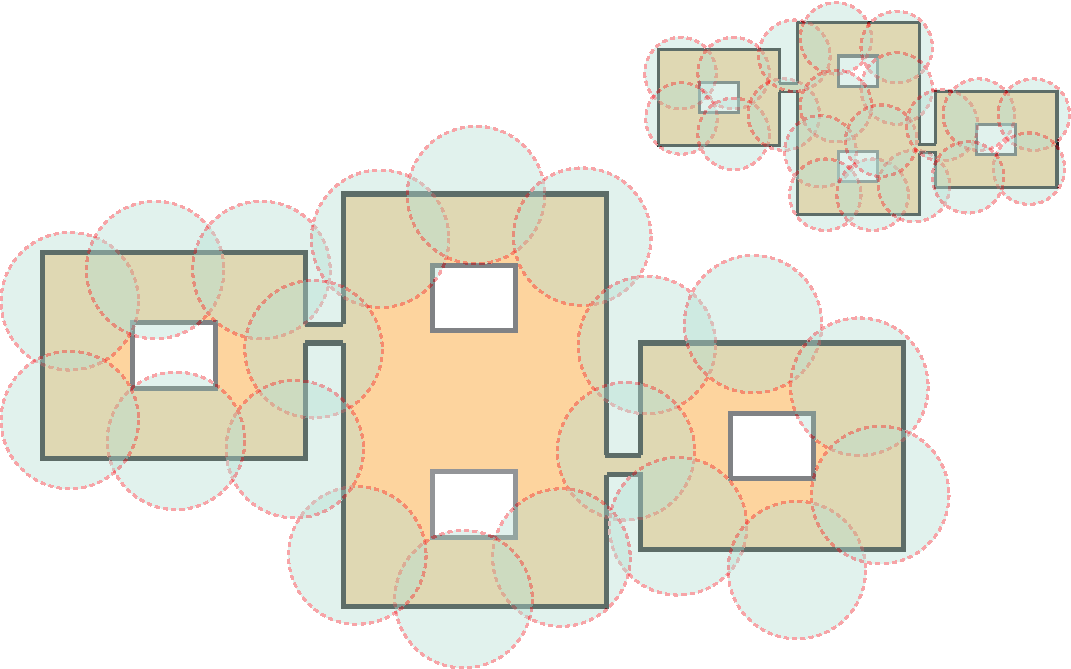
\includegraphics[width=\columnwidth]{chapters/osg/figures/example-0-eps-converted-to.pdf}
		\vspace*{1mm}
    \caption{An illustration of the \osgt setup and sample solutions.
		[center] The background shows the footprint of a building, e.g., an 
		apartment  complex. Scenarios may arise that a dangerous criminal 
		might be hiding in the building and we would like to closely monitor 
		the outer boundary of the building.	For the setting, the shaded 
		discs provide a	near-optimal cover with minimum radii for $20$ 
		mobile sensors that fully encloses the outer perimeter, computed 
		using algorithms presented in this work with optimality guarantees. 
		[upper right] A near-optimal solution for guarding the interior of
		the building footprint minus the four holes.}
    \label{fig:example0}
\end{figure}
As a summary of the study, on the side of computational complexity, we 
establish that \opgt is hard to approximate within a factor of 
$1.152$
even when the perimeter is a simple closed polygonal chain whose length
is bounded by the input size, through a reduction from 
vertex cover on planar bridgeless $3$-regular graphs.
%
A unique property of our reduction is that it shows the inapproximability gap
remains when each sensor can cover at most two disjoint perimeter 
segments. 
%
The proof also shows that \orgt is at least as hard to approximate. 
Therefore, no polynomial time algorithm may exist that solves \osgt to 
better than the $1.152$-optimal lower bound, unless P$\,=\,$NP. 
%
On the algorithmic side, we begin by providing an efficient $(1+\varepsilon)$
approximation algorithm
for a specific class of \opgt problems in which each mobile 
sensor must cover a continuous perimeter segment. This implies that the 
aforementioned inapproximability result on \opgt under the 
two-disjoint-segment sensing model is tight. 
%
For the general \osgt problem, we first describe a polynomial time 
$(2+\varepsilon)$ approximation algorithm as a reasonable approximability 
upper bound. 
%
Then, an integer linear programming (ILP) model is devised that allows 
the fast computation of highly optimal solutions for fairly large 
problem instances. 
%\jy{Maybe an example here on the scale of problems that we can solve and how fast.}
%
Results described in this paragraph, together with the introduction 
of \osgt as a practical multi-robot deployment problem focusing on global 
optimality, constitute the main contributions of this work. 

As an intermediate result toward showing the hardness of the simple polygon
coverage problem, we also supply a hardness proof of vertex cover 
on planar bridgeless\footnote{That is, the deletion of any edge does not disconnect 
the graph.} $3$-regular graphs, which may be of independent interest. 

\textbf{Related work}. Our work on optimal perimeter and region guarding 
draws inspiration from a long line of multi-robot coverage planning and 
control research, e.g., \cite{cortes2004coverage,martinez2007motion,
schwager2009optimal,pavone2009equitable,schwager2009decentralized,
pierson2017adapting}. 
%
In an influential body of work on coverage control \cite{cortes2004coverage,
martinez2007motion}, a gradient based iterative method is shown to drive 
one or multiple mobile sensors to a locally optimal configuration with 
convergence guarantees. 
%
Whereas \cite{cortes2004coverage,martinez2007motion} assume that the 
distribution of sensory information is available {\em a priori}, it is 
shown that such information can be effectively learned 
\cite{schwager2009decentralized}. 
%
Subsequently, the control method is further extended to allow the 
coverage of non-convex and disjoint 2D domains \cite{schwager2009optimal} 
and to work for mobile robots with varying sensing or actuation capabilities
\cite{pierson2017adapting}. 
%
In contrast to these control-based approaches, which produce iterative 
locally optimal solutions, \osgt emphasizes the direct computation of 
globally optimal deployment solutions and supports arbitrarily shaped
bounded (1D) perimeters and (2D) regions.

Recently, the problems of globally optimally covering perimeters using 
one-dimensional sensors have been studied in much detail 
\cite{fenghangaoyu2019efficient,fengyu2020RAL}. It is shown that when the sensors 
are homogeneous, the optimal deployment of sensors can be computed 
very efficiently, even for highly complex perimeters \cite{fenghangaoyu2019efficient}.
On the other hand, the problem becomes immediately intractable, sometimes
strongly NP-hard, when sensors are heterogeneous \cite{fengyu2020RAL}. 
Our research is distinct from \cite{fenghangaoyu2019efficient,fengyu2020RAL} in that 
we employ a (two-dimensional) range sensing model and work on the coverage 
of both perimeters and regions, which has much broader applicability. 

As pointed out in \cite{cortes2004coverage,schwager2009decentralized}, 
distributed sensor coverage, as well as \osgt, has roots in the study 
of the facility location optimization problem 
\cite{weber1929theory,drezner1995facility}, which examines the selection 
of facility (e.g., warehouses) locations that minimize the cost of delivery 
of supplies to spatially distributed customers. In theoretical computer 
science and operations research, these are known as the $k$-center, 
$k$-means, and $k$-median clustering problems \cite{har2011geometric}, 
the differences among which are induced by the cost structure. Our 
investigation of \osgt benefits from the vast literature on 
the study of $k$-center clustering and related problems, e.g., 
\cite{feder1988optimal,hochbaum1985best,gonzalez1985clustering,daskin2000new,shamos1975closest}.
%
These clustering problems are in turn related to packing 
\cite{hales2005proof}, tiling \cite{thue1910dichteste}, and the 
well-studied art gallery problems \cite{o1987art,shermer1992recent}.

\textbf{Organization}. The rest of the paper is organized as follows. 
In Section~\ref{sec:problem}, we introduce the \osgt formulation. 
Section~\ref{sec:complexity} is devoted to establishing that \osgt is 
hard to approximate to better than $1.152$-optimal, providing a theoretical
lower bound. In Section~\ref{sec:algo}, focusing on the upper bound, 
we describe algorithms that for \osgt and the special \opgt variant 
where a sensor is allowed to cover a continuous perimeter segment.
In Section~\ref{sec:expr}, we benchmark the algorithms and illustrate two 
potential applications. We discuss and conclude the work in Section~\ref{sec:conc}.





\section{Preliminaries}\label{sec:problem}
% We define .... 
Let $\mathcal{W}\subset \mathbb{R}^2$ be a 
% compact (i.e., closed and bounded) 
polygonal workspace, which may contain one or multiple connected components. 
A {\em critical subset} of $\mathcal{W}$ needs to be guarded by $k$ 
%\sw{jumpping from $r_i$ to inditinguishable}
indistinguishable point guards with range sensing capabilities. For 
example, the workspace may be a forest reserve and the critical subset 
may be its boundary. Or, the workspace may be a high-security facility, 
e.g., a prison, and the critical subset the prison yard. The $i$th 
guard, $1\le i\le k$, located at $c_i \in \mathbb{R}^2$, can monitor a circular 
area of radius $r_i$ centered at $c_i$ with $r_i$ being a variable. For 
example, the guard may be a watchtower equipped with a vision sensor 
that can detect intruders. As the watchtower's altitude increases, 
its sensing range also increases; but its monitoring quality will 
decrease at the same time due to resolution loss. In this study, we seek 
to compute the optimal strategy to deploy these $k$ guards so that the 
required sensing range, $\max_i r_i$, could be minimized. 

More formally, we model a connected component of $\W$ as some 2D polygonal region
containing zero or more simple polygonal obstacles. 
For a bounded set $D \subset \mathbb{R}^2$, we define
\begin{equation*}
size(k, D) = \min_{c_1, \dots, c_k\in \mathbb{R}^2}\ \max_{p\in D}\ \min_{1\leq i\leq k} \lVert c_i - p \rVert_2 
\end{equation*}
and use $B(c, r)$ to denote the disc of radius $r$ centered at a point $c 
\in \mathbb{R}^2$ (the definition of $size(k, D)$ is used extensively in later 
sections). 
Intuitively, $size(k,D)$ represents the minimum radius needed such that there
exisits $k$ circles with radius $size(k, D)$ that can cover the 2D bounded region $D$ entirely.
% The critical subset of interest in this work is either part of the boundary of $\W$, denoted $\partial \W$, or $\W$ itself. 
The main problem studied in this work is:

\begin{problem}[Optimal Set Guarding with 2D Sensors]
Given a polygonal workspace $\W \subset \mathbb{R}^2$, let $D \subset \W$ be a 
critical subset to be guarded by $k$ robots each with a variable coverage radius of $r$. Find 
the smallest $r$ and corresponding robot locations $c_1, \dots, c_k\in \mathbb{R}^2$, such that $D \subset \cup_i B(c_i, r)$.
\end{problem}

For making accurate statements about computational complexity, we make
the assumption that the length of $\partial \W$ is bounded by a polynomial with respect 
to the complexity of $\W$, (i.e. the number of vertices of the polygon). 
% Furthermore, we assume the possible 
% sensing radius of the robots is lower and upper bounded by some constants, 
% as is the case in practice. 

For convenience, we give specific names to these optimal guarding 
problems based critical subset types. If the critical 
subset belongs to $\partial \W$, we denote the problem as {\em optimal 
perimeter guarding with 2D sensors} or \opgt. If the critical subset 
is $\W$, we denote the problem as {\em optimal region guarding with 
2D sensors} or \orgt. When there is no need to distinguish, the problem 
is denoted as {\em optimal set guarding with 2D sensors} (\osgt). 
%The decision versions of \opgt and \orgt are denoted 
%\dopgt and \dorgt, respectively. 

As an example, to guard the boundary of a plus-shaped polygon with $5$ 
robots, an optimal solution could be ~\ref{fig:osg-example} where the 
inner circle covers $4$ disconnected boundary segments, such pattern 
in the optimal solution also renders \opgt much more difficult than 
the simplified 1D sensing model studied in \cite{fenghangaoyu2019efficient} 
(indeed, \opgt becomes hard to approximate, as will be shown shortly). 
The solution is also optimal under the \orgt formulation.
\begin{figure}[ht]
    \centering
		\vspace*{3mm}
    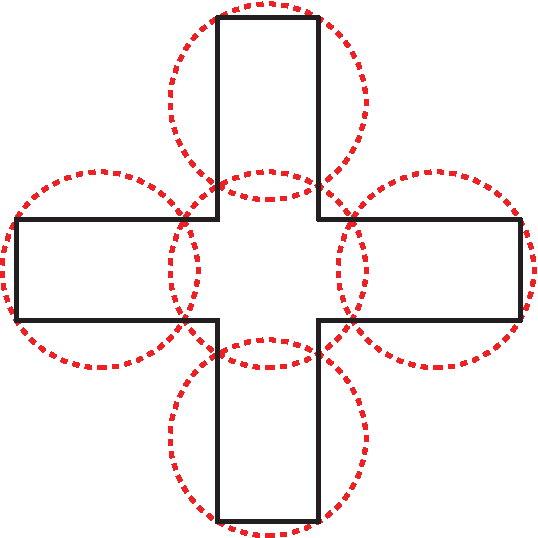
\includegraphics[scale=0.35]{chapters/osg/figures/exp_fig-e-eps-converted-to.pdf}
		\vspace*{1.5mm}
    \caption[An example showing an optimal solution of using five discs to cover the plus-shaped polygon]
    {An example showing an optimal solution of using five discs
		to cover the plus-shaped polygon. The solution is optimal for both 
		\opgt and \orgt formulations.}
    \label{fig:osg-example}
\end{figure}



\section{Computational Complexity for Variable Number of Robot Types}\label{sec:hardness}
We explore in this section the computational complexity of \opglr 
and \opgmc. Both problems are shown to be NP-hard with \opglr 
being strongly NP-hard. We later confirm that \opgmc is weakly 
NP-hard (in Section~\ref{sec:algorithm}).

\subsection{Strong NP-hardness of \opglr}\label{subsec:opglr-hardness}
When the number of types $t$ is a variable, i.e., $t$ is not a constant
and may be arbitrarily large,
% (but bounded by $n$), 
\opglr is shown to be NP-hard via the reduction from \tpart \cite{garey1975complexity}:

\vspace*{1mm}
\noindent
PROBLEM: \tpart\\
INSTANCE: A finite set A of $3m$ elements, a bound $B\in \mathbb{Z^+}$, 
% $S$ with $|S| = 3m$,
and a ``size'' $s(a)\in \mathbb{Z^+}$ for each $a\in A$,
such that each $s(a)$ satisfies $B/4 < s(a) <B/2$ and $\sum_{a\in A} s(a) = mB$.\\
QUESTION: Is there a partition of $S$ into $m$ disjoint subsets $S_1, 
\ldots, S_m$ such that for $1\leq i\leq m$, 
$\sum_{a\in S_i} s(a) = B$?
\vspace*{1mm}

%In a \tpart instance, let $\sum_{s \in S} s = B$ and for all $b \in B$, 
%$1/4 < b <  1/2$. Under such conditions, \tpart remains strongly 
%NP-hard \cite{garey1979computer}. We will use this version of the \tpart problem. We mention here that we use fractional values for 
%the elements of $B$ to avoid adding additional variables; this is fine 
%as long as we restrict the involved numbers to be rationals. 
\tpart is shown to be NP-complete in the strong sense\cite{GarJoh79}, 
i.e., it is NP-complete even when all numeric inputs are bounded by a polynomial 
of the input size. 

For the reduction, it is more convenient to work with a decision 
version of the \opglr problem, denoted as \opglrd. In the \opglrd 
problem, $a_{\tau}$ is the actual length robot type $\tau$ covers. 
That is, the coverage length of a robot is fixed. The \opglrd problem 
is specified as follows. 

\vspace*{1mm}
\noindent
PROBLEM: \opglrd\\
INSTANCE: $t$ types of robots where there are $n_{\tau}$ robots for 
each type $1 \le \tau \le t$; $n = n_1 + \cdots + n_t$. A robot of 
type $\tau$ has a coverage capacity $a_{\tau}$. A set of perimeters 
$\P = \{P_1, \ldots, P_m\}$ of a set of 2D regions 
$\R =\{R_1, \ldots, R_m\}$.\\ 
QUESTION: Is there a deployment of $n$ disjoint subsets $C_1, \ldots, C_n$
of $\{\partial R_1, \ldots, \partial R_m\}$ such that 
$P_1 \cup \ldots \cup P_m \subset C_1 \cup \ldots \cup C_n$, where
$C_j$ is a continuous segment for all $1 \le j \le n$, and for each 
$1 \le j \le n$, there is a unique robot whose type $\tau$, $1 \le \tau 
\le t$ satisfies $a_{\tau} \ge len(C_j)$?
\vspace*{1mm}

\begin{theorem}\label{t:opglr-hard}
	\opglr is strongly NP-hard. 
\end{theorem}
\begin{proof}
	A polynomial reduction from \tpart to \opglrd is constructed
	by a restriction of \opglrd. Given a \tpart instance with former notations,
	we apply several restrictions on \opglrd: {\em (i)} there are $3m$ types of robot
	and there is a single robot 
	for each type, i.e., $n_{\tau} = 1$ for $1 \le \tau \le t$, so $n=t=3m$ 
	{\em (ii)} the $3m$ capacities $a_1, \ldots, a_{3m}$ are set to be equal to
	$s(a)$ for each of the $3m$ elements $a\in A$, and {\em (iii)} 
	there are $3m$ perimeters and each perimeter $P_i$ is continuous and
	$len(P_i)=B$ for all $1 \le i \le m$.

	% \begin{comment}
	% In this proof, we work with a further restriction of \opglrd: {\em (i)}
	% there is a single robot for each type, i.e., $n_{\tau} = 1$ for $1 
	% \le \tau \le t$, and {\em (ii)} each perimeter $P_i$ is continuous and
	% %$len(P_i)$ is the same for all $1 \le i \le m$.
	
	% $len(P_i) = B$ for all $1 \le i \le m$.
	% Given a \tpart instance with $\sum_{b_i \in B} b = q$ and $1/4 \le b 
	% \le  1/2$ for all $b_i \in B$, let the corresponding \opglrd instance 
	% have $q$ perimeters, each with a single segment with the same length 
	% $L$. Let there be $3q$ robots, each with a type $1 \le \tau \le 3q$ 
	% and capability parameter $a_{\tau} = b_{\tau} \in B$. The restricted
	% \opglrd problem instance asks a question similar to the \tpart problem: 
	% is there a partition of the robots such that each perimeter of length 
	% $1$ is covered by three robots (notice that it is impossible to reach 
	% a total capacity of $1$ with fewer or more than $3$ robots)? 
	% \end{comment}

	% \begin{comment}
	% We make some rudimentary observations regarding the \opglrd instance 
	% and the related \opglr instance. Since all $q$ perimeters are of length 
	% $L$ each and the total capability of the robots is $q$, the objective 
	% \eqref{eq:objective} cannot be lower than $\frac{qL}{q} = L$, which is 
	% achieved only when each perimeter is covered by robots with total 
	% capability parameter of $1$. Then, because of the requirement $1/4 < 
	% a_{\tau} < 1/2$, if the best possible solution to the related \opglr 
	% instance is to be realized, each perimeter must be covered by exactly 
	% three robots; otherwise, the total capability cannot sum up to $1$. 
	% \end{comment}
	
	With the setup, the reduction proof is straightforward. Clearly, the 
	\tpart instance admits a partition of $A$ into $S_1, \ldots, 
	S_m$ such that $\sum_{a \in S_i} s(a) = B$ for all $1\leq i\leq m$ 
	if and only if a
	valid depolyment exists in the corresponding \opglrd instance. 
	It is clear that the reduction from \tpart to 
	\opglrd is polynomial (in fact, linear). Based on the 
	reduction and because \tpart is strongly NP-hard, so is \opglrd 
	%(by Lemma 4.1 of \cite{garey1975complexity}) 
	and \opglr.
\end{proof}

\begin{remark}
	One may also reduce weakly NP-hard problems, e.g., \twopart
	\cite{karp1972reducibility}, to \opglr for variable number of robot 
	types $t$. Being strongly NP-hard, \opglr is unlikely to admit pseudo-polynomial 
	time solutions for variable $t$. This contrasts with a later result 
	which provides a pseudo-polynomial time algorithm for \opglr for 
	constant $t$, as one might expect in practice where robots have limited 
	number of types. We also note that Theorem~\ref{t:opglr-hard} continues 
	to hold for a single perimeter with multiple segments, each 
	having a length $B$ in previous notation, separated by ``long'' gaps. Obviously, 
	\opglrd is in NP, thus rendering it NP-complete. 
\end{remark}

\subsection{NP-hardness of \opgmc}
The minimum cost \opg variant, \opgmc, is also NP-hard, which may be 
established through reduction from the \subsetsum problem 
\cite{karp1972reducibility}:

\vspace*{1mm}
\noindent
PROBLEM: \subsetsum \\
INSTANCE: A set $B$ with $|B| = n$ and a weight function $w: B \to 
\mathbb Z^+$, and an integer $W$.\\ 
QUESTION: Is there a subset $B' \subseteq B$ such that $\sum_{b \in B'} 
w(b) = W$?
\vspace*{1mm}

\begin{theorem}\label{t:opgmc-hard}
	\opgmc is NP-hard. 
\end{theorem}
\begin{proof}
	Given a \subsetsum instance, we construct an \opgmc instance with a 
	single perimeter containing a single segment with length $L$ to be 
	specified shortly. Let there be $t=2n$ types of robots. For $1 \le i 
	\le n$, let robot type $2i-1$ have $\ell_{2i-1} = c_{2i-1} = 
	w(b_i) + (2^{n + 1} + 2^i)W'$ and let robot type $2i$ have $\ell_{2i} 
	= c_{2i} = (2^{n + 1} + 2^i)W'$. Here, $W'$ can be any integer number no less than 
	$\sum_{b\in B} w(b)$. Set $L = W + (n2^{n+1} + 2^n + \ldots 
	+ 2^1)W'$. We ask the ``yes'' or ``no' decision question of whether there 
	are robots that can be allocated to have a total cost no more than $L$ 
	(equivalently, equal to $L$, as the cost density $c_\tau/l_\tau$
	is always $1$).
	
	Suppose the \subsetsum instance has a yes answer that uses a subset
	$B' \subseteq B$. Then, the \opgmc instance has a solution with cost $L$ 
	that can be constructed as follows. For each $1 \le i \le n$, a single 
	robot of type $2i - 1$ is taken if $b_i \in B'$. Otherwise, a single 
	robot of type $2i$ is taken. This allocation of robots yields a total 
	length and cost of $L$. 
	
	For the other direction, we first show that if the \opgmc instance 
	is to be satisfied, it can only use a single robot from type $2i-1$ 
	or $2i$ for all $1 \le i \le n$. First, if more than $n$ robots are 
	used, then the total cost exceeds $(n + 1)2^{n+1}W' > L$ as $W\leq W'$.
	% because $W' + (2^n + \ldots + 2)W' < 2^{n+1}W'$. 
	Similarly, if less than $n$ 
	robots are used, the total length is at most 
	$(n-1)2^{n+1}W'+(2^{n+1}-1)W'+ W' < L$. 
	Also, to match the $(2^n + \ldots + 2)W'$ part of the cost, exactly one robot 
	from type $2i-1$ or $2i$ for all $1 \le i \le n$ must be taken. 
	Now, if the \opgmc decision instance has a yes answer, if a robot 
	of type $2i -1$ is used, let $b_i \in B$ be part of $B'$, which 
	constructs a $B'$ that gives a yes answer to the \subsetsum instance.
\end{proof}
% add this citation because the proof the hardness probably comes from it
\begin{remark}
	It is also clear that the decision version of the \opgmc problem is 
	NP-complete. The \subsetsum is a weakly NP-hard problem that admits 
	a pseudo-polynomial time algorithm \cite{dantzig1957discrete}. 
	As it turns out, \opgmc, which shares similarities with \subsetsum
	and \ttkp (in particular, \ttukp \cite{ukphardness}), though NP-hard, 
	does admit a pseudo-polynomial time algorithm as well. 
\end{remark}

\begin{comment}
In concluding the section, we note that we have not determined the 
hardness for the case with constant number of robot types. There are 
some recent evidence that such problems may not be as hard as when 
the number of robot types is a fixed input parameter 
\cite{goemans2014polynomiality}.
\end{comment}



% \section{Exact Algorithm via Dynamic Programming}\label{sec:algorithm}
\section{Exact Algorithms for \opglr and \opgmc}\label{sec:algorithm}
\begin{comment}
\jy{We can be more precise with the section title. This is a balance between
brevity and level of detail. Generally, I try to fill one line; sometimes
I use two lines if I feel it needs that much detail.}
\end{comment}
In this section, we describe three exact algorithms for solving the two 
variations of the \opg problem. First, we present a pseudo-polynomial time
algorithm for \opglr when the number of robot types, $t$, is a fixed constant. 
Given that \opglr is strongly NP-hard, this is in a sense a best possible 
solution. 
%
For \opgmc, in addition to providing a pseudo-polynomial algorithm for 
arbitrary $t$, which confirms that \opgmc is weakly NP-hard, we also provide
a polynomial time approximation scheme (PTAS). We then further show the 
possibility of solving \opgmc in polynomial time when $t$ is a fixed constant. 
We mention that our development in this section focuses on the single 
perimeter case, i.e., $m = 1$, as the generalization to arbitrary $m$ is 
straightforward using techniques described in \cite{fenghangaoyu2019efficient}. With this in mind, 
we also provide the running times for the general setting with arbitrary $m$ 
but refer the readers to \cite{fenghangaoyu2019efficient} on how these running times can be derived. 

For presenting the analysis and results, for the a perimeter $P$ that we work 
with, assume that it has $q$ perimeter segments $S_1, \ldots, S_q$ that need 
to be guarded; these segments are separated by $q$ gaps $G_1, \ldots, G_q$. 
For $1 \le i, i' \le q$, define $S_{i\sim i'} = S_i \cup G_i \cup S_{i+1} \cup \ldots 
\cup G_{i'-1} \cup S_{i'}$ where $i'$ may be smaller than $i$ (i.e., $S_{i\sim i'}$
may wrap around $G_q$),
For the general case with $m$ perimeters, assume that a perimeter $P_i$ has
$q_i$ segments. 
\begin{comment}
\jy{A paper, or anything with some level of complexity to digest, should be 
hierarchical. So, at the beginning of a section, it is good to explain a bit 
of what will be covered so a reader will have an idea of the structure of 
the section.}
\end{comment}

\subsection{Pseudo-Polynomial Time Algorithm for \opglr with Fixed Number
of Robot Types}
\SetKw{Continue}{continue}
\SetKw{True}{true}
\SetKw{False}{false}
\SetKwComment{Comment}{\%}{}
\SetKwInOut{Input}{Input}
\SetKwInOut{Output}{Output}
\def\inc{{\sc Inc}\xspace}
\def\knapsack{\textbf{\textsc{Knapsack}}\xspace}
\def\opglrfeasible{{\sc OPG-lr-Feasible}\xspace}
\def\opgmcdp{{\sc OPG-mc-DP}\xspace}
We set to develop an algorithm for \opglr for arbitrary $t$, the number of robot 
types; the algorithm runs in pseudo-polynomial time when $t$ is a constant. 
At a higher level, our proposed algorithm works as follows. First, our main effort 
here goes into deriving a feasibility test for \opglrd as defined in 
Section~\ref{subsec:opgext-opglr-hardness}. With such a feasibility test, we can then 
find the optimal $\frac{len(C_j)}{a_{\tau_j}}$ in \eqref{eq:opgext-opg-objective} via binary search.
Let us denote the optimal value of $\frac{len(C_j)}{a_{\tau_j}}$ as $\ell^*$. 

\subsubsection{Feasibility Test for \opglrd} The feasibility test for \opglrd 
essentially tries different candidate $\ell$ to find $\ell^*$. Our implementation uses 
ideas similar to the pseudo-polynomial time algorithm for the \knapsack problem which
is based on dynamic programming (DP). In the test, we work with a fixed starting point on 
$P$, which is set to be the counterclockwise end point of a segment $S_i$, $1 \le i \le q$. 
Essentially, we maintain a $t$ dimensional array $M$ where dimension $\tau$
has a size of $n_{\tau} +1$. An element of the array, $M[n_1']\ldots[n_t']$, holds the 
maximal distance starting from $S_i$ that can be covered by $n_1'$ type 1 robots, 
$n_2'$ type 2 robots, and so on. The DP procedure \opglrfeasible($i, \ell$), outlined in 
Algorithm~\ref{algo:opgext-opglrd}, incrementally builds this array $M$. For convenience,
in the pseudo code, $M[\vec{x}]$ denotes an element of $M$ with $\vec{x}$ being 
a $t$ dimensional integer vector. 

\begin{algorithm}
	\DontPrintSemicolon
	% \KwData{$n_1, n_2, \cdots, n_k$ robots, $l_1, l_2, \cdots, l_n$ coverage distance}
	\KwData{$n_1, \ldots, n_t$, $a_1, \ldots, a_t$,
		$S_1, \ldots, S_q$, $G_1, \ldots, G_q$}
	\KwResult{\True or \False,  indicating whether $S_1, \ldots, S_q$ can be covered}
	%\Begin{
		Initialize $M$ as a $t$ dimensional array with dimension $\tau$ having a size of $n_{\tau} + 1$;\;
		$\ell_{\tau} \leftarrow a_{\tau}\ell$ for all $1\le \tau \le t$;\;
		\For{$ \vec{x} \in [0, n_1]\times\dots\times[0,n_t]$}{
            $M[\vec{x}]\leftarrow 0$;\;
			\For{$j = 1$ \KwTo $t$}{
				\lIf{$\vec{x}_j = 0$}{\Continue;}
				$\vec{x'}\leftarrow\vec{x}$; $\vec{x'}_j \leftarrow \vec{x'}_j - 1$;\;
				$M[\vec{x}]\leftarrow max$($M[\vec{x}]$, \inc($M[\vec{x'}], \ell_j$));\;
			}
			% \For{$i_2 \leftarrow 1$ \KwTo $n_2$}{
			% $\cdots$\;
			% \For{$i_k \leftarrow 1$ \KwTo $n_k$}{
			% $DP[i_1][i_2]\cdots[i_k]\leftarrow$ min(Increment($DP[i_1-1][i_2]\dots[i_k],\cdots,l_1$), Increment($DP[i_1][i_2-1]\dots[i_k], l_2$), $\cdots$, Increment($DP[i_1][i_2]\cdots[i_k-1],l_k$)\;
			% }
			% }
		}
		\Return{$M[n_1]\ldots[n_t] \ge len(S_{i\sim {i-1}})$};
	%}
	\caption{\opglrfeasible($i, \ell$)}\label{algo:opgext-opglrd}
\end{algorithm}

In Algorithm~\ref{algo:opgext-opglrd}, the procedure \inc($L, \ell$) checks how much of the 
perimeter $P$ can be covered when an additional coverage length $\ell$ is added, 
assuming that a distance of $L$ (starting from some $S_i$) is already covered. An 
illustration of how \inc($L, \ell$) works is given in ~\ref{fig:opgext-inc}.
 

\begin{figure}[ht]
	\begin{center}
		\begin{overpic}[width=0.7\textwidth,tics=5]
			{chapters/opg-ext/figures/inc-eps-converted-to.pdf}
			\put(26,10){{\small $L$}}
			\put(61,10){{\small $\ell$}}
			\put(30,1){{\small \textsc{Inc}($L$, $\ell$)}}
		\end{overpic}
	\end{center}
    \caption[Illustration of a solution]{\label{fig:opgext-inc}Suppose starting from the fixed left point, a 
		length of $L$ on the boundary is successfully guarded by a group of 
		robots. Then, a robot with coverage capacity $\ell$ is appended to 
		the end of the group of robots to increase the total guarded distance. 
		In the figure, the added additional capacity $\ell$ can fully cover 
		the third red segment plus part of the third (dashed) gap. Because 
		there is no need to cover the rest of the third gap, 
		\textsc{Inc}($L$, $\ell$) extends to the end of the gap.}
\end{figure}

%Denote procedure $Inc(L, \ell)$ as the length of boundary successfully guarded from $L$ using a continuous segment length of $\ell$.

%It is straightforward to see that Algorithm~\ref{algo:opglrd} has a running 
%time of $O(t\Pi_{i=1}^{t} (n_i+1))$ if we populate $M$ gradually.

By simple counting, the complexity of the algorithm is
$O(q\cdot t\cdot\Pi_{\tau=1}^{t} (n_{\tau}+1))$. However, the amortized
complexity of \inc($\cdot$) for each $\tau$ is $O(q+n_{\tau})$; the algorithm thus 
runs in $O(t\cdot\Pi_{{\tau}=1}^{t}(n_{\tau}+1)+q\cdot\sum_{{\tau}=1}^{t} 
\Pi_{{\tau'}\neq {\tau}} (n_{\tau'} +1))$, 
which is pseudo-polynomial for fixed $t$. After trying every possible starting 
position $i$ with \opglrfeasible($i, \ell$), for a fixed candidate $\ell$, 
\opglrd is solved in $O(q \cdot t\cdot\Pi_{{\tau}=1}^{t}(n_{\tau}+1) + 
q^2\cdot\sum_{{\tau}=1}^{t} \Pi_{{\tau'}\neq {\tau}} (n_{\tau'} +1))$.

\subsubsection{Solving \opglr using Feasibility Test for \opglrd}
Using \opglrfeasible($i, \ell$) as a subroutine to check feasibility for a given $\ell$, 
bisection can be applied over candidate $\ell$ to obtain $\ell^*$. For completing 
the algorithm, one needs to establish when the bisection will stop (notice that, 
even though we assume that $a_\tau \in \mathbb{Z^+}$, for each $1\leq \tau \leq t$, $\ell^*$ need not be 
an integer). 

To derive the stop criterion, we note that given the optimal $\ell^*$, there must 
exist some $S_{i\sim i'}$ that is ``exactly'' spanned by the allocated robots.
That is, assume that $S_{i\sim i'}$ is covered by $n_1'$ of type $1$ robots
and $n_2'$ of type $2$ robots, and so on, then 
\begin{align}\label{eq:opgext-exact}
\ell^* = \frac{len(S_{i\sim i'})}{\sum_{1 \le \tau \le t} a_{\tau}\cdot n_{\tau}'}.
\end{align}

\eqref{eq:opgext-exact} must hold for some $S_{i\sim i'}$ because if not, the solution 
is not tight and can be further improved. Therefore, the bisection process for 
locating $\ell^*$ does not need to go on further after reaching a certain granularity\cite{fenghangaoyu2019efficient}.
%$1/\sum_{1 \le \tau \le t} a_{\tau}\cdot n_{\tau}$. 
With this established, using 
similar techniques from \cite{fenghangaoyu2019efficient} (we omit the technical detail as it is quite 
complex but without additional new ideas beyond beside what is already covered 
in \cite{fenghangaoyu2019efficient}), we could prove that the full algorithm needs 
no more than $O(q\log(\sum_{\tau}n_{\tau}+q)$ calls to \opglrfeasible($i, \ell$).
%$O(t\Pi_{i=1}^{t}(n_i+1)+q\sum_{i=1}^{t} \Pi_{j\neq i} (n_j +1))$
This directly implies that \opglr also admits a pseudo-polynomial algorithm for fixed $t$.
% \sw{The complexity here is the decision version of single perimeters}
\subsubsection{Multiple Perimeters}
Also using techniques developed in \cite{fenghangaoyu2019efficient}, the single perimeter 
result can be readily generalized to multiple perimeters. We omit the mechanical
details of the derivation and point out that the computational complexity in this case becomes
$\tilde{O}( (m-1)\cdot((\Pi_{\tau=1}^t n_\tau) / \max_\tau n_\tau)^2 + 
\sum_{k=1}^{m} (t\cdot q_k\cdot \Pi_{{\tau}=1}^{t}(n_{\tau}+1)+
q_k^2\sum_{{\tau}=1}^{t} \Pi_{{\tau'}\neq {\tau}} (n_{\tau'} +1)))$.
% \sw{the complexity here is for decision version of multiple perimeters, starting
%  from a specific starting point}
%\jy{I updated the formula as it seems to be wrong. Also changed $r$ to $m$.}

\subsection{Polynomial Time Algorithm for \opgmc with Fixed Number of Robot Types}
%\subsection{$OPG_{MC}$}
The solution to \opgmc will be discussed here. A method based on DP 
will be provided first, which leads to a polynomial time algorithm for a 
fixed number of robot types and a pseudo-polynomial time algorithm when the number 
of robot types is not fixed. For the latter case, a polynomial time approximation 
scheme (PTAS) will also be briefly described.
\subsubsection{Dynamic Programming Procedure for \opgmc}
\def\sol{{\sc Sol}}
\def\presol{{\sc PreSolve}}
When no gaps exist, the optimization problem becomes a covering 
problem as follows. Let $c_{\tau}$, $\ell_{\tau}$, $n_{\tau}$ correspond to the cost, 
coverage length, and quantity of robot type ${\tau}$, respectively, and let total 
length to cover be $L$. We are to solve the optimization problem
\begin{align}\label{eq:opgext-ip}
    \min \sum_{\tau} c_{\tau} \cdot n_{\tau} \quad s.t.\, \quad
    \sum_{\tau} \ell_{\tau} \cdot n_{\tau} \geq L, n_{\tau}\geq 0.
\end{align}

Let the solution to the above integer programming problem be \sol($L$).
Notice that, for $S_{i\sim i'}:=\{S_i,\ G_i, \dots, 
G_{i'-1}, S_{i'}\}$, the minimum cost cover is by either: {\em (i)} 
covering the total boundary without skipping any gaps, 
%
or {\em (ii)} skipping or partially covering some gap, for example $G_k, 
i \le k \le j-1$.
%
In the first case, the minimum cost is exactly \sol$(\lceil len(S_{i\sim(i+k)}\rceil)$.
%
In the second case, the optimal structure for the two subsets of perimeter 
segments $S_{i\sim k}$ and $S_{(k+1)\sim j}$ still holds. This means that the 
continuous perimeter segments $S_{i\sim j}$ can be divided into two parts, 
each of which can be treated separately. This leads to a DP approach for \opgmc.
With $M[i][j]$ denoting the minimum cost to cover $S_{i\sim j}$, the DP recursion 
is given by
\[
	\scalebox{0.93}{$M[i][j] = \min(\textit{\sol}(\lceil len(S_{i\sim j})\rceil), \displaystyle\min_k(M[i][k]+M[k+1][j]))$}
\]

The DP procedure is outlined in Algorithm~\ref{alg:opgext-opgmc}. In the pseudo code, 
it is assumed that indices of $M$ are modulo $q$, e.g., $M[2][q+1] 
\equiv M[2][1]$. $tmp$ is a temporary variable. 
\begin{comment}
\jy{Generally mathematicians and theoretical computer scientists use 
	$\ell_1, \ldots, \ell_t$ instead of $\ell_1, \ell_2, \ldots, \ell_t$. The later is more 
	redundant. Also, normally we use ldots instead of cdots. I changed $C$ to $M$ since 
    $C$ is used elsewhere. I changed $==$ to $=$ to save space.}
\end{comment}
\begin{algorithm}
    \DontPrintSemicolon
    % \KwData{$n_1, n_2, \cdots, n_k$ robots, $l_1, l_2, \cdots, l_n$ coverage distance}
    \KwData{$\ell_1, \dots, \ell_t$, $c_1, \ldots, c_t$,
    	$S_1, \ldots, S_q$, $G_1, \ldots, G_q$}
    \KwResult{$c^*$, the minimum covering cost}
   %\Begin{
    $M \leftarrow$ a $q\times q$ matrix; $c^* \leftarrow \infty$; \;
    \For{$k \leftarrow 0$ \KwTo $q-1$}{
        \For{$i\leftarrow 1 $ \KwTo $q$}{
            $tmp \leftarrow\ $\sol$(\lceil len(S_{i\sim(i+k)}) \rceil)$; \;
            \For{$j\leftarrow i$ \KwTo $i+k-1$}{
                $tmp \leftarrow \min(tmp, M[i][j] + M[j+1][i+k])$;
            }
            $M[i][i+k] \leftarrow c$;\;
            \lIf{$k = q-1$}{$c^* \leftarrow \min(c^*, M[i][i+k])$;}
        }
    }
    \Return{$c^*;$}
    %}
    \caption{\opgmcdp}
    \label{alg:opgext-opgmc}
\end{algorithm}

\subsubsection{A Polynomial Time Algorithm for \opgmc for a Fixed Number of Robot Types}
We mention briefly that, by a result of Lenstra \cite{lenstra1983integer}, the optimization problem 
~\eqref{eq:opgext-ip} is in P (i.e., polynomial time) when $t$ is a constant. The running time of 
the algorithm \cite{lenstra1983integer} is however exponential in $t$. 

\subsubsection{A Pseudo-polynomial Time Algorithm for Arbitrary $t$}
As demonstrated in the hardness proof, similarities exist between \opg and the \knapsack 
problem. The connection actually allows the derivation of a pseudo-polynomial time algorithm
for arbitrary $t$. To achieve this, we use a routine to pre-compute \sol($L$), called 
\presol(), which is itself a DP procedure similar to that for the \knapsack problem. The 
pseudo code of \presol() is given in Algorithm~\ref{algo:opgext-presol}.
\presol() runs in time $O(t\cdot\lceil len(\partial R)\rceil))$. Overall, 
Algorithm~\ref{alg:opgext-opgmc} then runs in time $O(q^3+t\cdot\lceil len(\partial R\rceil))$.
%\jy{Is this running time correct?}

\begin{algorithm}
	\DontPrintSemicolon
	\KwData{$\ell_1, \ldots, \ell_t$, $c_1, \ldots, c_t$}
	\KwResult{A lookup table for retrieving \sol($L$)}
	%\Begin{
		$I_{max} = \lceil len(\partial R)\rceil$; \Comment{\small $I_{max}$ is an integer.}
		$M' \leftarrow$ an array of length $I_{max} + 1$; 
		$M'[0]\leftarrow 0$;\;
		\For{$L \leftarrow$ $1$ \KwTo $I_{max}$}{
			$M'[L]\leftarrow \infty$; \;
			\For{${\tau}\leftarrow 1$ \KwTo $t$}{
				$tmp \leftarrow (L<\ell_{\tau}\ ?\ 0\ :\ M'[L-\ell_{\tau}]) + c_{\tau}$;\;
				$M'[L] \leftarrow min(M'[L], tmp)$;\;
			}
		}
		\Return{$M'$}
	%}
	\caption{{\sc PreSolve}}\label{algo:opgext-presol}
\end{algorithm}

%After the preprocessing, 
%the Solution(L) is just an access of $Sol[L]$. 
%Algorithm \ref{alg:opgmc} still applies and the only modification is a simple replacement of 
%\sol($L$) with $Sola[L]$. This make the complexity of \ref{alg:opgmc} drop to $O(q^3)$.
% \begin{algorithm}
%     \DontPrintSemicolon
%     % \KwData{$n_1, n_2, \cdots, n_k$ robots, $l_1, l_2, \cdots, l_n$ coverage distance}
%     \KwData{$l_1, l_2, \cdots, l_k$ coverage distance, $c_1, c_2,\cdots,c_k$ deployment cost}
%     \KwResult{Minimum cost for covering the perimeter}
%     \Begin{
%     $DP \leftarrow$ 1-D array length of L with data initialized to $\infty$\;
%     $DP[0]\leftarrow 0 $\;
%     $Result\leftarrow \infty$\;
%     \For{$l \leftarrow 0$ \KwTo $L$}{
%     \If{$DP[l] = \infty$}{  \Continue\;}
%     \For{$i \leftarrow 1$ \KwTo $k$}{
%     $nextEnd \leftarrow $Increment($l, l_i$)\;
%     $DP[nextEnd] = \min(DP[nextEnd], DP[l]+c_i)$\;
%     \If{$nextEnd\geq L$}{Result$\leftarrow \min(Result,DP[nextEnd])$}
%     }
%     }
%     \Return{Result}
%     }
%     \caption{} 
% \end{algorithm}
With the establishment of a pseudo-polynomial time algorithm for \opgmc, we  
have the following corollary. 
\begin{corollary}
	\opgmc is weakly NP-hard. 
\end{corollary}

\subsubsection{FPTAS for Arbitrary $t$}
When the number of robot types is not fixed, Lenstra's algorithm\cite{lenstra1983integer} or 
its variants no longer run in polynomial time. We briefly mention that, 
%via a linear time transformation, 
by slight modifications of a FPTAS for \ttukp problem from \cite{ibarra1975fast}, a FPTAS 
for \opgmc can be obtained that runs in time $O(q^3 + q^2 \cdot \frac{t}{\epsilon^3})$, 
where $(1+\epsilon)$ is the approximation ratio for both \opgmc and ~\eqref{eq:opgext-ip}. 

\subsubsection{Multiple Perimeters} For \opgmc, when there are multiple 
perimeters, e.g., $P_1, \ldots, P_m$, a optimal solution can be obtained 
by optimally solving \opgmc for each perimeter $P_i$ individually and 
then put together the solutions. 



%\section{Experimental Studies}\label{sec:experiments}
%\input{texs/05-experiments}

\section{Performance Evaluation and Applications}\label{sec:application}
In this section, we provide examples illustrating the typical 
optimal solution structures of \opglr and \opgmc computed by 
our DP algorithms. Using an application scenario, solutions to 
\opglr and \opgmc are also compared. Then, computational 
results from extensive numerical evaluations are presented, 
confirming the effectiveness of these algorithms. The 
implementation is done using the Python and all 
computations are performed on an Intel(R) Core(TM) i7-7700 CPU@3.6GHz 
with 16GB RAM. 

\subsection{Basic Optimal Solution Structure}
Fig.~\ref{fig:opgext-opglrm} shows the typical outcome of solving an \opglr 
instance with two perimeters ($m = 2$) for two types of robots with 
$n_1 = 3, a_1 = 5$, and $n_2 = 5, a_2 = 8$. 
%That is, the second type of robots is more capable than the first type. 
In the figure, the red segments are parts of the two perimeters that 
must be guarded. The three orange (resp., five green) segments across 
the two perimeters indicate the desired coverage regions of the three 
(resp., five) type $1$ (resp., type $2$) robots. These coverage regions 
correspond to the optimal solution returned by the DP algorithm. As 
may be observed, the optimal solution is somewhat complex with robots 
of both types on each of the two perimeters; a gap on the second boundary 
also gets covered. The coverage lengths for a robot type are generally 
different; this is due to adjustments that shrink some robots' coverage. 
For example, the first perimeter has a very short orange cover because 
the corresponding perimeter segment is short and gaps around it need 
not be covered (The adjustment procedure is also shown in the video). 
\begin{figure}[!ht]
    \centering
    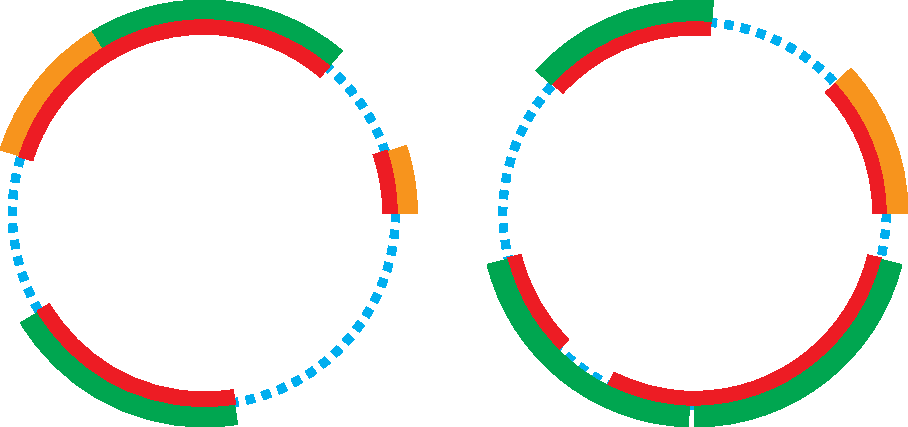
\includegraphics[scale = 0.6]{chapters/opg-ext/figures/mopglr_shrink-new-eps-converted-to.pdf}
    \caption{An \opglr problem and an associated optimal solution. The 
		problem has two perimeters and $t = 2$ with $n_1$=3, $n_2$=5, 
		$a_1$=5, $a_2$=8. The boundaries are shown as circles for ease of 
		illustration.
		%, which does not affect the computation or the solution.
		}
		\label{fig:opgext-opglrm}
\end{figure}

Shifting our attention to \opgmc, Fig.~\ref{fig:opgext-opgmc} illustrates the 
structure of an optimal solution to a problem with three types of robots 
with capacities and costs being $\ell_1=11, c_1=2$, $\ell_t=30, 
c_2=4$, and $\ell_3=55, c_3=7$, respectively. In this case, the majority 
of the deployed robots are of type $2$ with $\ell_2=30, c_2=4$. Only one 
type $1$ and one type $3$ robots are used. The four perimeter segments are 
covered by three robot groups. 
%
%To clearly illustrate the solution structure, the combined coverage of each 
%robot group runs beyond the counterclockwise direction of the corresponding 
%segments being covered (e.g., the counterclockwise end of the orange segment 
%is inside a gap). 
%
The only type $3$ robot guards (the purple segment) across two different 
perimeter segments. Coverage length adjustment is also performed to avoid 
the unnecessary coverage of some gaps. 

\begin{figure}[!ht]
    \centering
    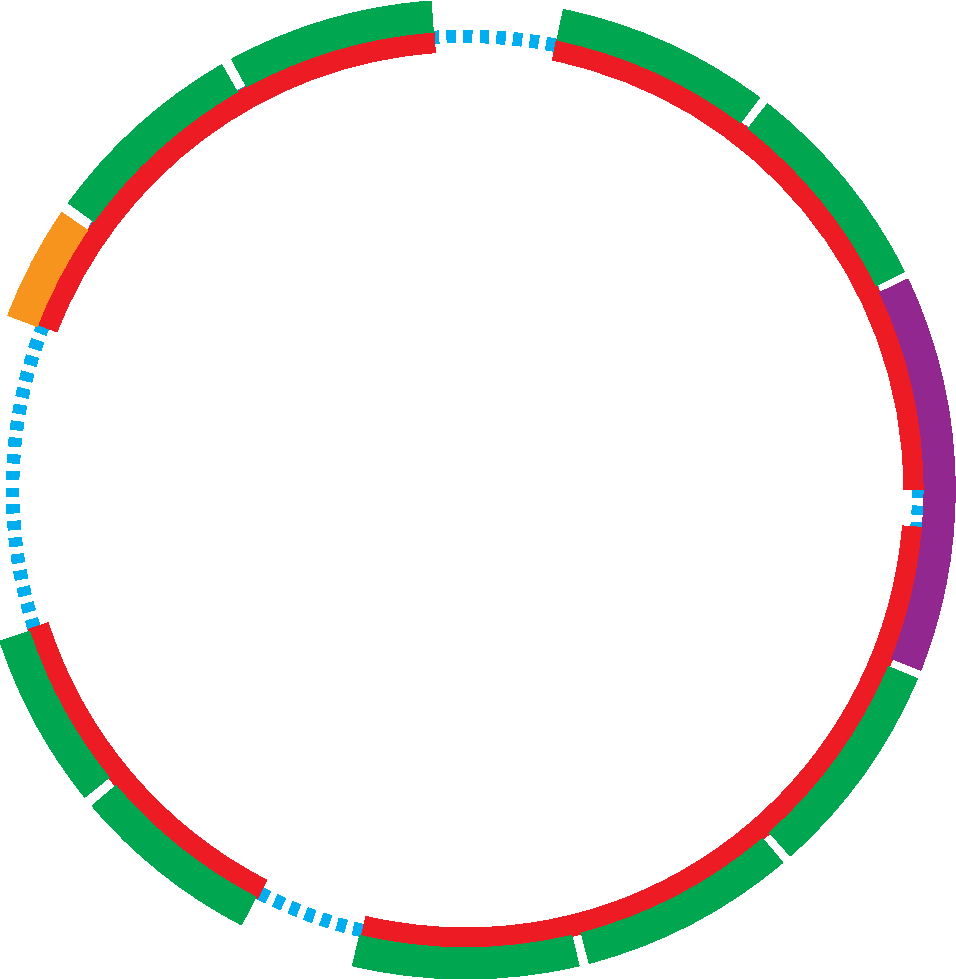
\includegraphics[scale = 0.4]{chapters/opg-ext/figures/opgmc-new-t-eps-converted-to.pdf}
    \caption{An \opgmc problem and an associated optimal solution. The 
		problem has four (red) perimeter segments and three types of robots
		with $\ell_1=11, c_1=2$ (orange), $\ell_t=30, c_2=4$ (green), 
		and $\ell_3=55, c_3=7$ (purple), respectively.}
		\label{fig:opgext-opgmc}
\end{figure}

\subsection{A Robotic Guarding and Patrolling Application}
In this subsection, as a potential application, the DP algorithms for 
\opglr and \opgmc are employed to solve the problem of securing the 
perimeter of the Edinburgh castle, an example used in 
\cite{FenHanGaoYu19RSS}. As shown in Fig.~\ref{fig:opgext-castle} (minus 
the orange and green segments showing the solutions), the central 
region of the Edinburgh castle has tall buildings on its boundary 
(the blocks in brick red); these parts of the boundary are the gaps 
that do not need guarding. In the figure, the top sub-figure shows 
the optimal solution for an \opglr instance and an \opgmc instance with 
a total of $11$ robots. The bottom sub-figure is a slightly updated 
\opgmc instance with slightly higher $c_2$. 
\begin{figure}[!ht]
    \centering
    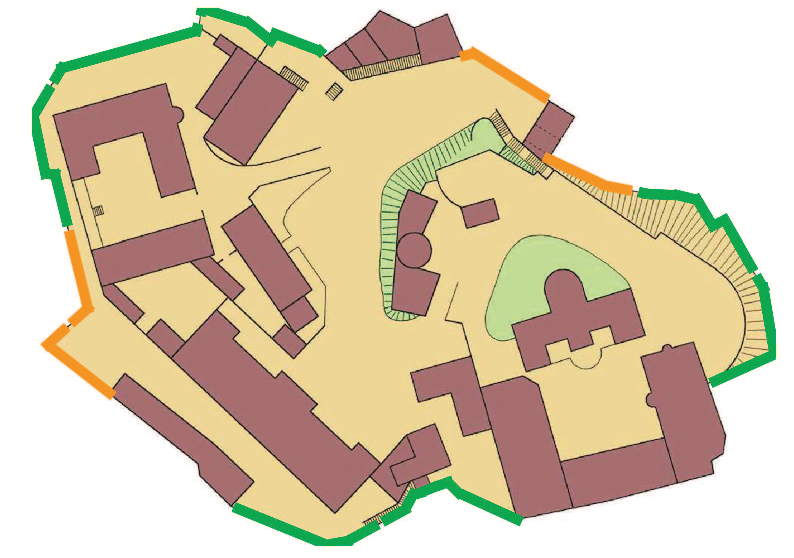
\includegraphics[scale = 0.5]{chapters/opg-ext/figures/opglr-castle-thin-eps-converted-to.pdf}
    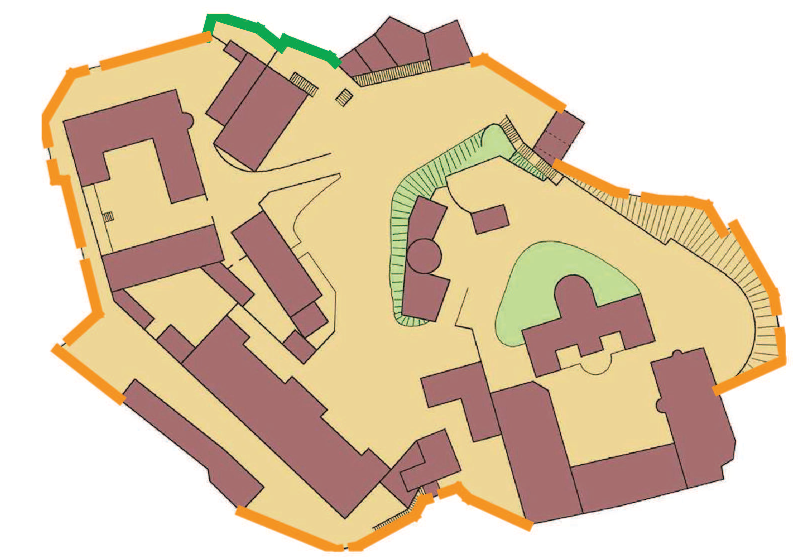
\includegraphics[scale = 0.5]{chapters/opg-ext/figures/opgmc-castle-thin-eps-converted-to.pdf}
    \caption{[left] \opglr solution with $n_1 = 4, n_2 = 7, 
		c_1:c_2 = 2:3$ and \opgmc solution with $\ell_1 = 150, 
		c_1 = 100, \ell_2 = 225, c_2 = 145$, and total boundary $3058$. Cost 
		of \opgmc solution is $1415$.
		[right] \opgmc solution with $\ell_1 = 150, c_1 = 100, \ell_2 = 
		225, c_2 = 155$. Cost of solution ($13$ type $1$, $1$ type $2$) is 
		$1455$.
		%
		In both solutions, covers by type $1$ (resp., 
		type $2$) robots are shown in orange (resp., green).
		%, which does not affect the computation or the solution.
		}
		\label{fig:opgext-castle}
\end{figure}

It can be observed that the results, while having non-trivial structures, 
make intuitive sense. For the top sub-figure, solutions to both \opglr 
and \opgmc (because robot with larger capacity is slightly lower in 
relative cost) use mainly higher capacity robots to cover longer perimeter 
segments and use the lower capacity robots mostly fillers. The solution 
covers a small gap at the bottom. For the bottom sub-figure, while only 
small changes are made to the cost, because the longer segment is more 
expensive to use now, the first type of robot is used mainly. 

\subsection{Computational Performance}
With Section~\ref{sec:opgext-algorithm} fully establishing the correctness and 
asymptotic complexity of the pseudo-polynomial time algorithms, here, the 
running time of these algorithms are experimentally evaluated. In doing 
so, the main goal is demonstrating that, despite the hardness of \opglr 
and \opgmc, the proposed algorithms could solve the target problems under 
reasonably broad settings in a scalable way. For results presented in 
this subsection, each data point is an average over 10 randomly generated 
instances. 

The first two numerical evaluations (Table~\ref{tab:opgext-opglr} and 
Table~\ref{tab:opgext-mopglr}) focus on the running times of the pseudo-polynomial 
time algorithms for \opglr over single and multiple perimeters, 
respectively. In these two tables, $t$ and $q$ are the number of types 
and the number of segments, respectively. For each type $\tau$, a 
capacity ($a_{\tau}$) is randomly sampled as an integer between $1$ and 
$100$, inclusive. The number of robots available for each type ($n_{\tau}$) 
is sampled uniformly between $5$ and $15$, inclusive. For the multiple 
perimeters case, the parameter $m$ represents the number of perimeters for 
a given instance.

For the single perimeter case (Table~\ref{tab:opgext-opglr}), the results show 
that the pseudo-polynomial time algorithm is effective for up to five 
types of robots, for dozens of robots. We expect a more efficient 
(e.g., C++ based) implementation should be able to effectively handle 
up to five types of robots with the total number of robots being around 
a hundred, on a typical PC. This is likely sufficient for many practical 
applications which have limited types and numbers of robots. Since the 
algorithm has exponential dependency on $t$, it becomes less efficient 
for larger $t$ as expected.  

\begin{table}[htbp]
	\centering
	\begin{tabularx}{\columnwidth}{|c|X|X|X|X|X|X|}
		\hline
%		\renewcommand{\arraystretch}{0.99}
		\diagbox{$t$}{$q$}&  \quad 5 &   \quad 10 &\quad 20& \quad 30 & \quad 40&\quad 50 \\
		\hline
		\renewcommand{\arraystretch}{1.05}
		2&0.022 &0.044 &0.131 &0.208 &0.326 &0.516 \\\hline
        3&0.281 &0.714 &1.670 &2.577 &4.107 &4.708 \\\hline
        4&5.504 &16.07 &41.68 &71.55 &109.9 &138.9 \\\hline
        5&29.53 &75.60 &243.6 &443.4 &528.0 &725.0 \\\hline
	\end{tabularx}
	\caption{Running time in seconds used by the DP algorithm for \opglr over 
	a single perimeter.
	}
	\label{tab:opglr}
\vspace*{-1mm}
\end{table}

Table~\ref{tab:opgext-mopglr} illustrates the running time of the DP algorithm for 
\opglr over multiple perimeters. As can be readily observed, the impact of 
the number of perimeters $m$ on the running time is relatively small; the 
number of robot types is still the determining factor for running time. In 
this case, our proposed solution is effective for $t$ up to $4$ and starts to 
slow down a robot types become larger than $4$. 
\begin{table}[htbp]
	\centering
	\renewcommand{\arraystretch}{1.05}
    \begin{tabularx}{\columnwidth}{|c|X|X|X|X|X|X|}
        \hline
        {\multirow{2}{*}{\diagbox{$m$}{$q$}} }&\multicolumn{2}{c|}{10}&\multicolumn{2}{c|}{20}&\multicolumn{2}{c|}{30} \\
        \cline{2-7}
         &\,\,\,$t$=3 & $\,\,\,t$=4& $\,\,\,t$=3 & $\,\,\,t$=4& \,\,\,$t$=3  & \,\,\,$t$=4\\
        \hline
        2&3.148 &133.2 &7.077 &198.4 &10.33 &260.0 \\\hline
        3&4.828 &194.1 &10.125 &290.6 &15.52 &376.7 \\\hline
        4&6.131 &256.8 &12.485 &381.3 &19.75 &514.3 \\\hline
        5&7.622 &321.7 &15.355 &476.2 &24.31 &605.8 \\\hline
    \end{tabularx}
    \caption{Running time in seconds used by the DP algorithm for \opglr over multiple perimeters.}
    \label{tab:mopglr}
\vspace*{-1mm}
\end{table}

Table~\ref{tab:opgext-opgmc} provides performance evaluation of \opgmcdp. Since 
there is no difference between single and multiple perimeters for \opgmc,
only problems with single perimeters are attempted. Here, for each robot 
type, the cost is an integer randomly sampled between $1$ and $20$, and 
the capacity is computed as five times the cost plus a random integer 
between $1$ and $20$. In the table, $L = \partial R$, the total length 
of the entire boundary. 
%
Given \opgmc's lower computational complexity, the DP algorithm, 
\opgmcdp, can effectively deal with over a few hundred types of robots 
with ease. 
\begin{table}[!ht]
	\centering
	\renewcommand{\arraystretch}{1.04}
    \begin{tabularx}{\columnwidth}{|c|X|X|X|X|X|X|}
        \hline
        \multirow{2}{*}{\diagbox{$t$}{$L$}} & 
        \multicolumn{2}{c|}{$10^2$}&\multicolumn{2}{c|}{$10^4$} &\multicolumn{2}{c|}{$10^6$} \\
        \cline{2-7}
        &$q$=20&$q$=50&$q$=20&$q$=50&$q$=20&$q$=50\\
        \hline
        3&0.006 &0.064 &0.041 &0.098 &3.040 &3.144 \\\hline
        10&0.005 &0.066 &0.094 &0.155 &9.423 &9.409 \\\hline
        30&0.009 &0.070 &0.261 &0.320 &26.10 &28.59 \\\hline
        100&0.014 &0.077 &0.910 &0.969 &91.28 &93.20 \\\hline
        300&0.030 &0.091 &2.652 &2.938 &275.6 &270.7 \\\hline
    \end{tabularx}
    \caption{Running time in seconds used by \opgmcdp algorithm.}
    \label{tab:opgext-opgmc}
\end{table}
\vspace*{-1mm}
\begin{comment}
    Application 1: for a single large region with a perimeter that may be viewed as straight line segments locally, we want to deploy multiple types of robots with different sensing radius. The goal is to ensure full coverage of the perimeter. Both problems formulations can be used. 

This also raises a related problem: what if we want to use discs to cover perimeter when a segment cannot be treated as straight lines? Can we also do tiling somehow? 

Another question: if we just use the same number of robots as used in an optimal cover to do a random feasible tiling, what would be the worst sub-optimality ratio? 

Application 2:  a multi-region application?
\end{comment}

\section{Conclusion and Discussions}\label{sec:conclusion}
In this section, we investigate two natural models of optimal perimeter 
guarding using heterogeneous robots, where one model (\opglr) limits 
the number of available robots and the second (\opgmc) seeks to 
optimize the total cost of coverage. 

These formulations have many potential applications. One application 
scenario we envision is the deployment of multiple agents or robots 
as ``emergency responders'' that are constrained to travel on the 
boundary. An optimal coverage solution will then translate to minimizing 
the maximum response time anywhere on the perimeter (the part that 
needs guarding). The scenario applies to \opg, \opglr, and \opgmc. 

Another application scenario is the monitoring of the perimeter 
using robots with different sensing capabilities. A simple heterogeneous 
sensing model here would be robots equipped with cameras with different 
resolutions, which may also be approximated as discs of different radii. 
The model makes sense provided that the region to be covered is much 
larger than the sensing range of individual robots and assuming that the 
boundary has relatively small curvature as compared to the inverse of the 
radius of the smallest sensing disc of the robots. For boundary with 
relatively small curvature, our solutions would apply well to the sensing 
model by using the diameter of the sensing disc as the 1D sensing range. 
As the region to be covered is large, covering the boundary will require
much fewer sensors than covering the interior. 


On the computational complexity 
side, we prove that both \opglr and \opgmc are NP-hard, with \opglr 
directly shown to be strongly NP-hard. This is in stark contrast to 
the homogeneous case, which admits highly efficient low polynomial 
time solutions \cite{fenghangaoyu2019efficient}. The complexity study also 
establishes structural similarities between these problems and 
classical NP-hard problems including \tpart, \ttkp, and \subsetsum.

On the algorithmic side, we provide methods for solving both \opglr 
and \opgmc exactly. For \opglr, the algorithm runs in pseudo-polynomial 
time in practical settings with limited types of robots. In 
this case, the approach is shown to be computationally effective. 
For \opgmc, a pseudo-polynomial time algorithm is derived for the 
general problem, which implies that \opgmc is weakly NP-hard. In 
practice, this allows us to solve large instances of \opgmc. We 
further show that a polynomial time algorithm is possible for 
\opgmc when the types of robots are fixed. 

With the study of \opg \cite{fenghangaoyu2019efficient} for homogeneous and 
heterogeneous cases, some preliminary understanding has been 
obtained on how to approach complex 1D guarding problems. 
Nevertheless, the study so far is limited to {\em one-shot} settings
where the perimeters do not change. In future research, we would like 
to explore the more challenging case where the perimeters evolve 
over time, which requires the solution to be dynamic as well. Given 
the results on the one-shot settings, we expect the dynamic setting
to be generally intractable if global optimal solutions are desired, 
potentially calling for iterative and/or approximate solutions. 

We recognize that our work 
does not readily apply to a visibility-based sensing model, which is also 
of interest. Currently, we are also exploring covering of the interior
using range-based sensing. As with the OPG work, we want to push for 
optimal or near-optimal solutions when possible.
\vspace*{-1mm}


% \newpage
\bibliographystyle{IEEEtran}
\bibliography{../bib/bib}

\end{document}